\section{Approach}

In the next section we describe our solution for the distributed lighting problem. The main components of our system are the Local Controller, used to maintain the illuminance at each desk at the desired reference, the Simplex Algorithm, that calculates the optimal solution to the linear programm that describes this problem, and the TCP/IP Server, which serves as an intermediary between the clients and the system. An overview of the system is depicted on Figure \ref{fig:global_system}.

\begin{figure}[!ht]
    \centering
        \includegraphics[scale=0.8]{img/GlobalSystem}
    \caption{Block diagram of the implemented system}\label{fig:global_system}
\end{figure}

\section{Physical Setup}
\label{sec:PhysicalSetup}

\subsection{System Characteristics}
\label{sec:SystemCharacteristics}

\subsubsection{Steady State}
\label{sub:SteadyState}

\begin{figure}[h]
    \centering
    \resizebox{\textwidth}{!}{% Title: glps_renderer figure
% Creator: GL2PS 1.3.8, (C) 1999-2012 C. Geuzaine
% For: Octave
% CreationDate: Tue Dec 29 01:06:44 2015
\setlength{\unitlength}{1pt}
\begin{picture}(0,0)
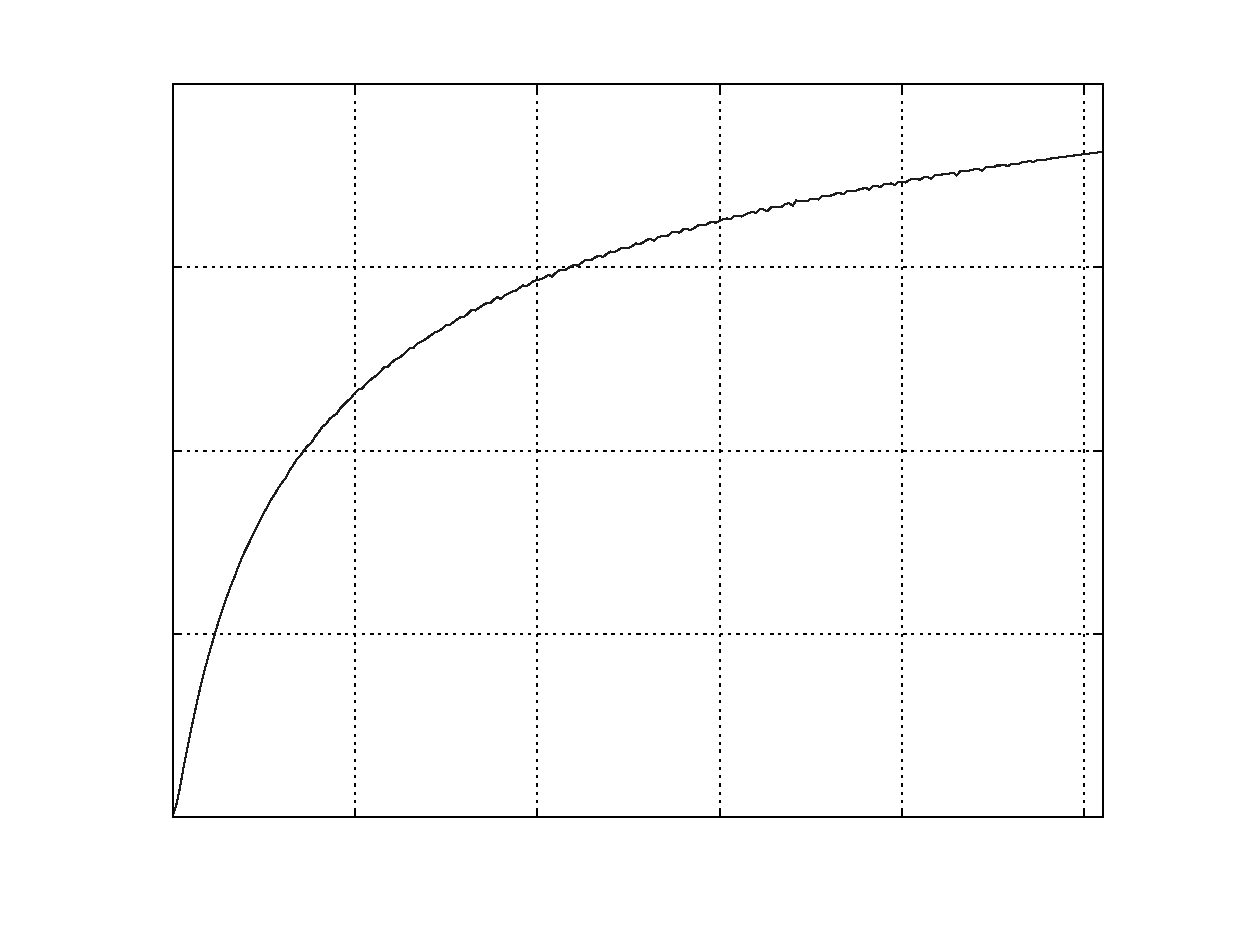
\includegraphics{img/steady_state-inc}
\end{picture}%
\begin{picture}(576,432)(0,0)
\fontsize{10}{0}
\selectfont\put(74.88,42.5189){\makebox(0,0)[t]{\textcolor[rgb]{0,0,0}{{0}}}}
\fontsize{10}{0}
\selectfont\put(162.409,42.5189){\makebox(0,0)[t]{\textcolor[rgb]{0,0,0}{{50}}}}
\fontsize{10}{0}
\selectfont\put(249.939,42.5189){\makebox(0,0)[t]{\textcolor[rgb]{0,0,0}{{100}}}}
\fontsize{10}{0}
\selectfont\put(337.468,42.5189){\makebox(0,0)[t]{\textcolor[rgb]{0,0,0}{{150}}}}
\fontsize{10}{0}
\selectfont\put(424.998,42.5189){\makebox(0,0)[t]{\textcolor[rgb]{0,0,0}{{200}}}}
\fontsize{10}{0}
\selectfont\put(512.527,42.5189){\makebox(0,0)[t]{\textcolor[rgb]{0,0,0}{{250}}}}
\fontsize{10}{0}
\selectfont\put(69.8755,47.52){\makebox(0,0)[r]{\textcolor[rgb]{0,0,0}{{0}}}}
\fontsize{10}{0}
\selectfont\put(69.8755,135.54){\makebox(0,0)[r]{\textcolor[rgb]{0,0,0}{{1}}}}
\fontsize{10}{0}
\selectfont\put(69.8755,223.56){\makebox(0,0)[r]{\textcolor[rgb]{0,0,0}{{2}}}}
\fontsize{10}{0}
\selectfont\put(69.8755,311.58){\makebox(0,0)[r]{\textcolor[rgb]{0,0,0}{{3}}}}
\fontsize{10}{0}
\selectfont\put(69.8755,399.6){\makebox(0,0)[r]{\textcolor[rgb]{0,0,0}{{4}}}}
\fontsize{10}{0}
\selectfont\put(298.08,31.5188){\makebox(0,0)[t]{\textcolor[rgb]{0,0,0}{{PWM value (0--255)}}}}
\fontsize{10}{0}
\selectfont\put(59.8755,223.56){\rotatebox{90}{\makebox(0,0)[b]{\textcolor[rgb]{0,0,0}{{Voltage at \texttt{A0} (\si{\volt})}}}}}
\end{picture}
}
    \caption{}
    \label{fig:}
\end{figure}

\begin{figure}[h]
    \centering
    \resizebox{\textwidth}{!}{% Title: glps_renderer figure
% Creator: GL2PS 1.3.8, (C) 1999-2012 C. Geuzaine
% For: Octave
% CreationDate: Tue Dec 29 00:54:08 2015
\setlength{\unitlength}{1pt}
\begin{picture}(0,0)
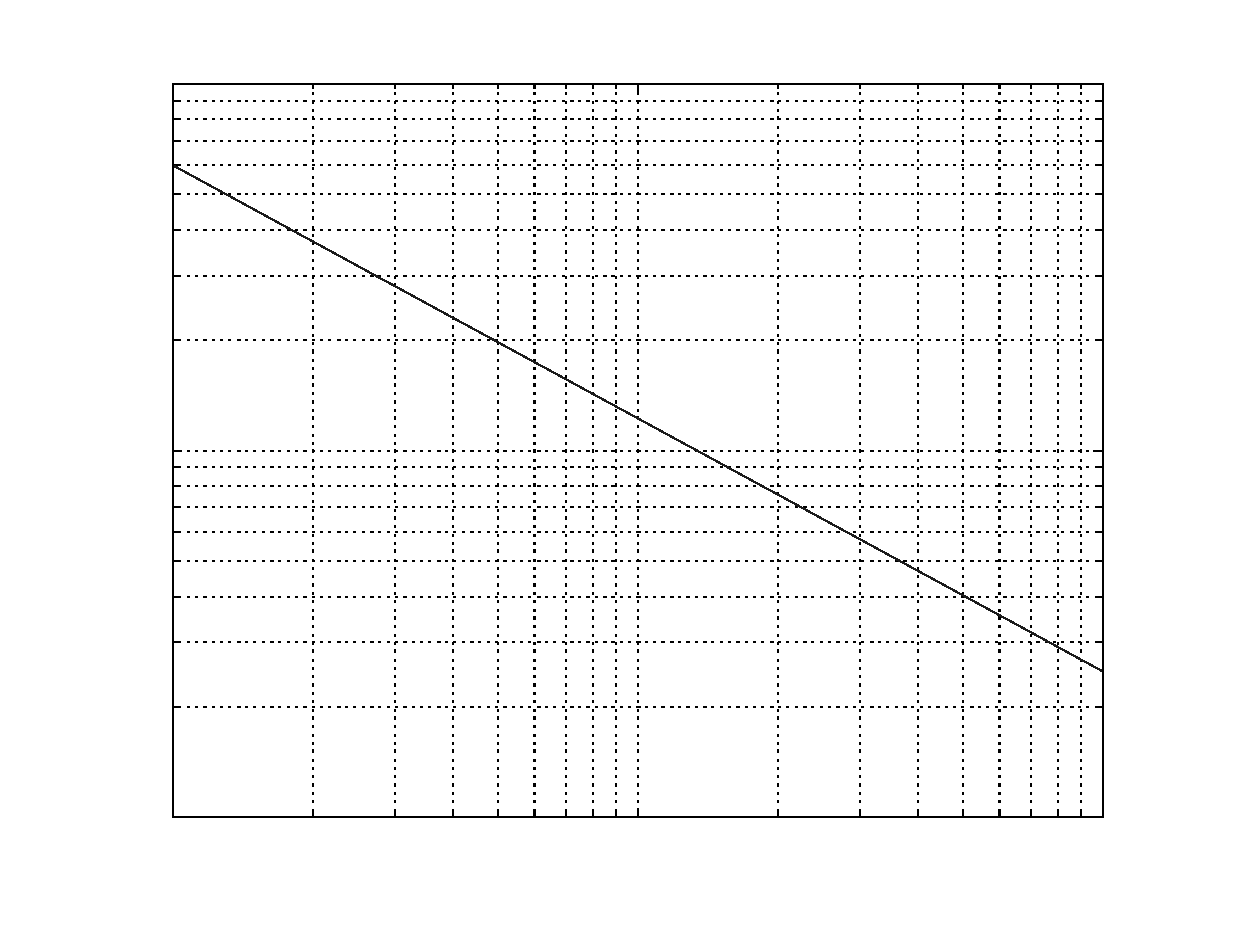
\includegraphics{img/LDR_model-inc}
\end{picture}%
\begin{picture}(576,432)(0,0)
\fontsize{10}{0}
\selectfont\put(74.88,42.5189){\makebox(0,0)[t]{\textcolor[rgb]{0,0,0}{{1e+0}}}}
\fontsize{10}{0}
\selectfont\put(298.08,42.5189){\makebox(0,0)[t]{\textcolor[rgb]{0,0,0}{{1e+1}}}}
\fontsize{10}{0}
\selectfont\put(521.28,42.5189){\makebox(0,0)[t]{\textcolor[rgb]{0,0,0}{{1e+2}}}}
\fontsize{10}{0}
\selectfont\put(69.8755,47.52){\makebox(0,0)[r]{\textcolor[rgb]{0,0,0}{{1e+3}}}}
\fontsize{10}{0}
\selectfont\put(69.8755,223.56){\makebox(0,0)[r]{\textcolor[rgb]{0,0,0}{{1e+4}}}}
\fontsize{10}{0}
\selectfont\put(69.8755,399.6){\makebox(0,0)[r]{\textcolor[rgb]{0,0,0}{{1e+5}}}}
\fontsize{10}{0}
\selectfont\put(298.08,31.5188){\makebox(0,0)[t]{\textcolor[rgb]{0,0,0}{{Illuminance (\si{\lux})}}}}
\fontsize{10}{0}
\selectfont\put(39.8755,223.56){\rotatebox{90}{\makebox(0,0)[b]{\textcolor[rgb]{0,0,0}{{Resistance (\si{\ohm})}}}}}
\end{picture}
}
    \caption{}
    \label{fig:}
\end{figure}

\subsubsection{Step Response}
\label{sub:StepResponse}

\subsubsection{Incremental Response}
\label{sub:IncrementalResponse}

\subsubsection{LDR to Lux}
\label{sub:LDRtoLux}

\begin{figure}[h]
    \centering
    \resizebox{\textwidth}{!}{% Title: glps_renderer figure
% Creator: GL2PS 1.3.8, (C) 1999-2012 C. Geuzaine
% For: Octave
% CreationDate: Tue Dec 29 00:58:25 2015
\setlength{\unitlength}{1pt}
\begin{picture}(0,0)
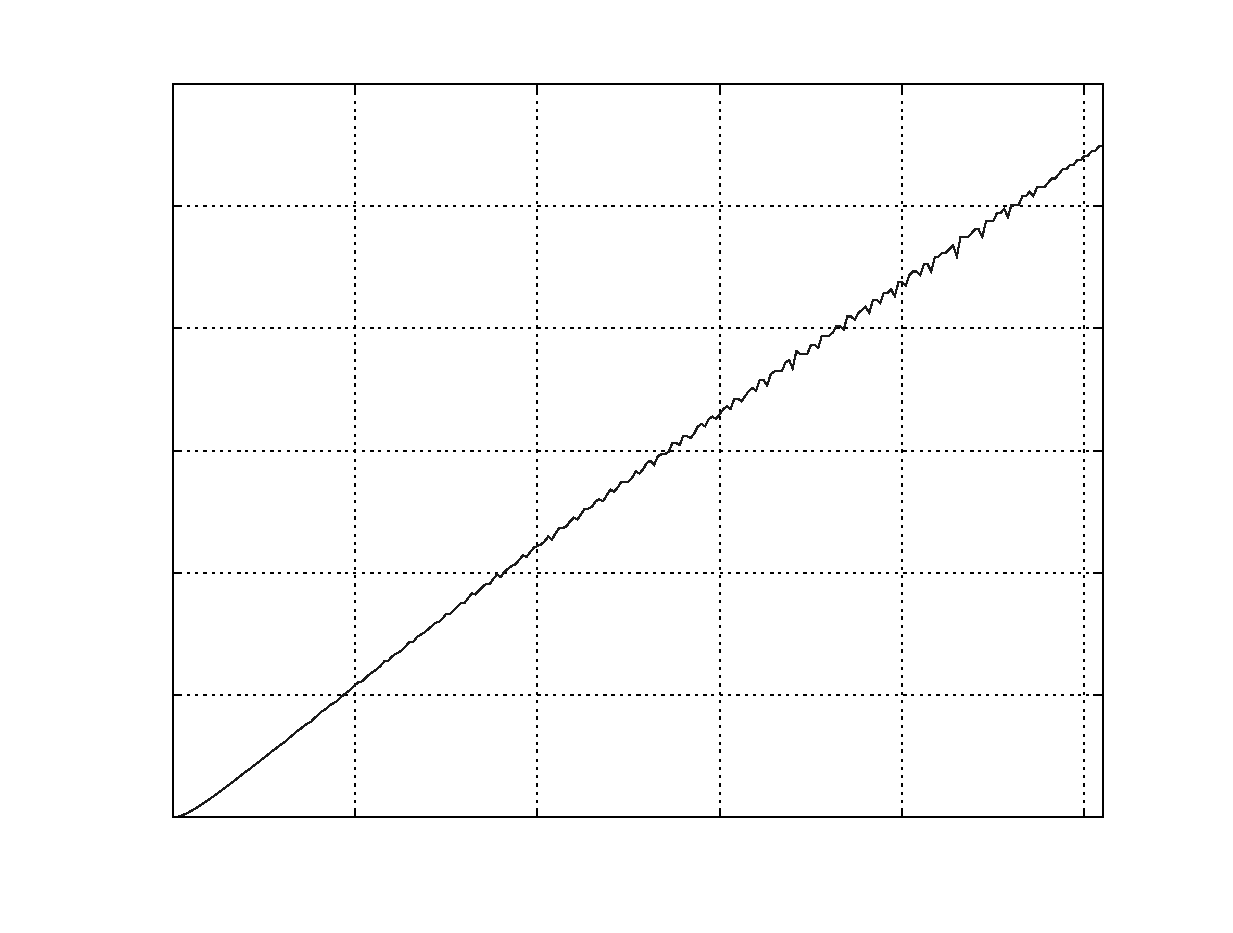
\includegraphics{img/pwm_to_lux-inc}
\end{picture}%
\begin{picture}(576,432)(0,0)
\fontsize{10}{0}
\selectfont\put(74.88,42.5189){\makebox(0,0)[t]{\textcolor[rgb]{0,0,0}{{0}}}}
\fontsize{10}{0}
\selectfont\put(162.409,42.5189){\makebox(0,0)[t]{\textcolor[rgb]{0,0,0}{{50}}}}
\fontsize{10}{0}
\selectfont\put(249.939,42.5189){\makebox(0,0)[t]{\textcolor[rgb]{0,0,0}{{100}}}}
\fontsize{10}{0}
\selectfont\put(337.468,42.5189){\makebox(0,0)[t]{\textcolor[rgb]{0,0,0}{{150}}}}
\fontsize{10}{0}
\selectfont\put(424.998,42.5189){\makebox(0,0)[t]{\textcolor[rgb]{0,0,0}{{200}}}}
\fontsize{10}{0}
\selectfont\put(512.527,42.5189){\makebox(0,0)[t]{\textcolor[rgb]{0,0,0}{{250}}}}
\fontsize{10}{0}
\selectfont\put(69.8755,47.52){\makebox(0,0)[r]{\textcolor[rgb]{0,0,0}{{0}}}}
\fontsize{10}{0}
\selectfont\put(69.8755,106.2){\makebox(0,0)[r]{\textcolor[rgb]{0,0,0}{{10}}}}
\fontsize{10}{0}
\selectfont\put(69.8755,164.88){\makebox(0,0)[r]{\textcolor[rgb]{0,0,0}{{20}}}}
\fontsize{10}{0}
\selectfont\put(69.8755,223.56){\makebox(0,0)[r]{\textcolor[rgb]{0,0,0}{{30}}}}
\fontsize{10}{0}
\selectfont\put(69.8755,282.24){\makebox(0,0)[r]{\textcolor[rgb]{0,0,0}{{40}}}}
\fontsize{10}{0}
\selectfont\put(69.8755,340.92){\makebox(0,0)[r]{\textcolor[rgb]{0,0,0}{{50}}}}
\fontsize{10}{0}
\selectfont\put(69.8755,399.6){\makebox(0,0)[r]{\textcolor[rgb]{0,0,0}{{60}}}}
\fontsize{10}{0}
\selectfont\put(298.08,31.5188){\makebox(0,0)[t]{\textcolor[rgb]{0,0,0}{{PWM value (0--255)}}}}
\fontsize{10}{0}
\selectfont\put(53.8755,223.56){\rotatebox{90}{\makebox(0,0)[b]{\textcolor[rgb]{0,0,0}{{Measured illuminance (\si{\lux})}}}}}
\end{picture}
}
    \caption{}
    \label{fig:}
\end{figure}


% From first report:

%Os seguintes pontos descrevem o que é implementado no código actual:
%Controlador com componentes proporcional, derivativa e integral
%Anti-windup
%Feedforward
%Derivador à saída
%Temporização do controlador através de interrupções
%Dar referências em lux
%Medir iluminância em lux
%Alterar parâmetros do controlador
%Alterar tempo de amostragem
%Implementamos um filtro passa-baixo para o derivador para diminuir o ruído. Não chegámos a afinar a constante desse filtro, pelo que o temos comentado.
%Os parâmetros do controlador foram encontrados com afinação manual e são os seguintes:
%Ganho proporcional: 10
%Ganho diferencial: 0.01
%Ganho integral: 10
%Ganho do feedforward: 0.1
%Ganho do anti-windup: 0.05
%Tempo de amostragem: 1500 µs
%Todos os cálculos do controlador são feitos com valores de 0 a 1023, sendo convertidos quando necessário: para 0 a 255 para actuar o LED; e para lux quando são pedidos valores de iluminância.

\subsection{Local Controller}
\label{sec:LocalController}

The local controller consists of a Proportional-Integral-Derivative Controller (PID) that receives as input a integer reference value (\emph{r}) from 0 to 1023, the LDR readings from 0 to 1023 (\emph{y}) and has as output the PWM duty cycle (\emph{u}) in the range 0 to 255.

The block diagram of the local controller is on Figure~\ref{fig:pid_block_diagramm}. The error(\emph{e}) is defined as $e = r - y$. The signal \emph{u} is calculated as the sum of the proportional, integral and derivative components and the feedforward term.

\begin{figure}[!h]
	\centering
		\includegraphics[scale=0.8]{img/pid_block_diagramm}
	\caption{Locall controller block diagram}\label{fig:pid_block_diagramm}
\end{figure}


\subsubsection{Proportional Component}
\label{sub:ProportionalComponent}

The proportional component of the controller is just a gain multiplied (\emph{$K_p$}) by \emph{e}. $ P = K_p * e$.

\subsubsection{Integral Component}
\label{sub:IntegralComponent}

\subsubsection{Derivative Component}
\label{sub:Derivative Component}

The derivative component is calculated as $ D = - K_d/T_s * (y_{t}-y_{t-1})$. This component is calculated with signal \emph{y} instead of \emph{u} to avoid differentiating discontinuities, which would cause the signal \emph{u} to saturate.

\subsubsection{Anti-Windup}
\label{sub:AntiWindup}

\subsubsection{Feedforward}
\label{sub:Feedforward}

\subsubsection{Implementation Details}
\label{sub:Implementation Details}

This controller was implemented as a interrupt routine to guarantee its execution in fixed intervals.

\subsubsection{Parameters}
\label{sub:Parameters}

\subsection{Server}
\label{sec:Server}

\subsection{Simplex}
\label{sec:Simplex}

The Simplex algorithms solves Linear programms, it finds the optimal solution if it exists.
We implemented the simplex following the pseudo-code on the book \emph{Introduction to Algorithms} \cite{Cormen}.
This implementation solves Linear programms of the form:

$$ \text{max }c*x $$
$$    A*x \geq b, $$
$$    x \geq 0 $$

We can describe the problem as a Linear programm of this form. First we define \emph{O} as the array with the external illuminance at each \emph{desk}, \emph{l} as the array with the desired illuminance for each \emph{desk} and \emph{E} as the  3 by 3 matrix of influence between each light. The problem we want to solve is to find the minimal values for \emph{d}, the PWM values normalized from 0 to 1, that make the illuminance be equal to \emph{l}.


Note: To throughly test the Simplex implementation a series of simple unit tests were constructed using the \emph{Boost Test} Library.

\subsection{Serial Communications}
\label{sec:SerialCommunications}

